% ============================================================
% Question Bank: ch06-02 Reproducing Scale Drawings at a Different Scale
% Topic Title: Reproducing Scale Drawings at a Different Scale
% CCSS: 7.G.A.1
% Questions: 27 (15 MC + 6 SA + 6 Graphical)
% ============================================================

% --- Multiple Choice Questions (15) ---

\begin{practiceQuestion}{6-2-q01}{mc}
\begin{questionText}
A map uses $1$ cm $= 40$ km. You redraw it at $1$ cm $= 20$ km. A river that is $5$ cm long on the original map becomes how long on the new map?
\end{questionText}
\choiceA{$2.5$ cm}
\choiceB{$5$ cm}
\choiceC{$10$ cm}
\choiceD{$100$ cm}
\correctAnswer{C}
\explanation{Scale ratio: $\frac{40}{20} = 2$. New length: $5 \times 2 = 10$ cm. The new scale is more detailed, so the drawing is larger.}
\end{practiceQuestion}

\begin{practiceQuestion}{6-2-q02}{mc}
\begin{questionText}
A floor plan uses $1$ cm $= 6$ m. You redraw it at $1$ cm $= 12$ m. A wall that is $8$ cm on the original becomes how long?
\end{questionText}
\choiceA{$2$ cm}
\choiceB{$4$ cm}
\choiceC{$8$ cm}
\choiceD{$16$ cm}
\correctAnswer{B}
\explanation{Scale ratio: $\frac{6}{12} = \frac{1}{2}$. New length: $8 \times \frac{1}{2} = 4$ cm. Larger scale means smaller drawing.}
\end{practiceQuestion}

\begin{practiceQuestion}{6-2-q03}{mc}
\begin{questionText}
A model uses scale $1:150$. You rebuild it at scale $1:50$. A doorway that is $2$ cm on the original becomes how long?
\end{questionText}
\choiceA{$0.67$ cm}
\choiceB{$2$ cm}
\choiceC{$6$ cm}
\choiceD{$300$ cm}
\correctAnswer{C}
\explanation{Scale ratio: $\frac{150}{50} = 3$. New length: $2 \times 3 = 6$ cm. Switching to a smaller ratio enlarges the model.}
\end{practiceQuestion}

\begin{practiceQuestion}{6-2-q04}{mc}
\begin{questionText}
A drawing uses $1$ cm $= 5$ m. It is redrawn at $1$ cm $= 15$ m. A hallway that is $9$ cm on the original becomes how long?
\end{questionText}
\choiceA{$3$ cm}
\choiceB{$9$ cm}
\choiceC{$27$ cm}
\choiceD{$45$ cm}
\correctAnswer{A}
\explanation{Scale ratio: $\frac{5}{15} = \frac{1}{3}$. New length: $9 \times \frac{1}{3} = 3$ cm.}
\end{practiceQuestion}

\begin{practiceQuestion}{6-2-q05}{mc}
\begin{questionText}
When you redraw a scale drawing at a larger scale (fewer real units per cm), the new drawing is:
\end{questionText}
\choiceA{Smaller than the original}
\choiceB{The same size as the original}
\choiceC{Larger than the original}
\choiceD{A different shape than the original}
\correctAnswer{C}
\explanation{A larger scale means each centimeter represents fewer real units, so more centimeters are needed to represent the same distance. The drawing gets bigger, but the shape stays the same.}
\end{practiceQuestion}

\begin{practiceQuestion}{6-2-q06}{mc}
\begin{questionText}
A map uses $1$ cm $= 16$ km. You redraw it at $1$ cm $= 4$ km. What happens to each length on the drawing?
\end{questionText}
\choiceA{It is divided by $4$}
\choiceB{It stays the same}
\choiceC{It is multiplied by $4$}
\choiceD{It is multiplied by $12$}
\correctAnswer{C}
\explanation{Scale ratio: $\frac{16}{4} = 4$. Every length is multiplied by $4$ on the new drawing because each centimeter now represents fewer real km.}
\end{practiceQuestion}

\begin{practiceQuestion}{6-2-q07}{mc}
\begin{questionText}
A blueprint uses $1$ cm $= 3$ ft. You redraw at $1$ cm $= 1$ ft. A room is $4$ cm by $5$ cm on the original. What is the area on the new drawing?
\end{questionText}
\choiceA{$20$ cm$^2$}
\choiceB{$60$ cm$^2$}
\choiceC{$100$ cm$^2$}
\choiceD{$180$ cm$^2$}
\correctAnswer{D}
\explanation{Scale ratio: $\frac{3}{1} = 3$. New dimensions: $4 \times 3 = 12$ cm and $5 \times 3 = 15$ cm. New area: $12 \times 15 = 180$ cm$^2$.}
\end{practiceQuestion}

\begin{practiceQuestion}{6-2-q08}{mc}
\begin{questionText}
A drawing uses scale $1:300$. It is redrawn at scale $1:150$. How does the area on the new drawing compare to the original?
\end{questionText}
\choiceA{It is $2$ times as large}
\choiceB{It is $4$ times as large}
\choiceC{It is $\frac{1}{2}$ as large}
\choiceD{It is the same}
\correctAnswer{B}
\explanation{Scale ratio: $\frac{300}{150} = 2$. Lengths double, so area is multiplied by $2^2 = 4$.}
\end{practiceQuestion}

\begin{practiceQuestion}{6-2-q09}{mc}
\begin{questionText}
A map uses $1$ cm $= 24$ km. A forest is $5$ cm wide on this map. You redraw at $1$ cm $= 6$ km. How wide is the forest on the new map?
\end{questionText}
\choiceA{$1.25$ cm}
\choiceB{$10$ cm}
\choiceC{$20$ cm}
\choiceD{$30$ cm}
\correctAnswer{C}
\explanation{Scale ratio: $\frac{24}{6} = 4$. New width: $5 \times 4 = 20$ cm.}
\end{practiceQuestion}

\begin{practiceQuestion}{6-2-q10}{mc}
\begin{questionText}
A floor plan uses $1$ in $= 8$ ft. You redraw at $1$ in $= 2$ ft. A window that is $0.75$ in on the original becomes how wide?
\end{questionText}
\choiceA{$0.75$ in}
\choiceB{$1.5$ in}
\choiceC{$3$ in}
\choiceD{$6$ in}
\correctAnswer{C}
\explanation{Scale ratio: $\frac{8}{2} = 4$. New width: $0.75 \times 4 = 3$ in.}
\end{practiceQuestion}

\begin{practiceQuestion}{6-2-q11}{mc}
\begin{questionText}
Which of the following does NOT change when a scale drawing is redrawn at a different scale?
\end{questionText}
\choiceA{The distances on the drawing}
\choiceB{The area of the drawing}
\choiceC{The angles in the figures}
\choiceD{The size of the drawing}
\correctAnswer{C}
\explanation{When the scale changes, lengths and areas change, but angles and proportions remain the same. The shapes are similar.}
\end{practiceQuestion}

\begin{practiceQuestion}{6-2-q12}{mc}
\begin{questionText}
A map uses $1$ cm $= 18$ km. A second map uses $1$ cm $= 9$ km. A highway is $6$ cm long on the first map. How long is it on the second?
\end{questionText}
\choiceA{$3$ cm}
\choiceB{$12$ cm}
\choiceC{$6$ cm}
\choiceD{$54$ cm}
\correctAnswer{B}
\explanation{Scale ratio: $\frac{18}{9} = 2$. New length: $6 \times 2 = 12$ cm.}
\end{practiceQuestion}

\begin{practiceQuestion}{6-2-q13}{mc}
\begin{questionText}
A drawing uses $1$ cm $= 4$ m. It is redrawn at $1$ cm $= 2$ m. The original drawing is $7$ cm by $3$ cm. What is the perimeter of the new drawing?
\end{questionText}
\choiceA{$20$ cm}
\choiceB{$40$ cm}
\choiceC{$42$ cm}
\choiceD{$84$ cm}
\correctAnswer{B}
\explanation{Scale ratio: $\frac{4}{2} = 2$. New dimensions: $7 \times 2 = 14$ cm and $3 \times 2 = 6$ cm. Perimeter: $2(14 + 6) = 40$ cm.}
\end{practiceQuestion}

\begin{practiceQuestion}{6-2-q14}{mc}
\begin{questionText}
Original scale: $1$ cm $= 8$ m. New scale: $1$ cm $= 32$ m. What is the scale ratio?
\end{questionText}
\choiceA{$\frac{1}{4}$}
\choiceB{$4$}
\choiceC{$24$}
\choiceD{$\frac{1}{24}$}
\correctAnswer{A}
\explanation{Scale ratio: $\frac{8}{32} = \frac{1}{4}$. Every old measurement is multiplied by $\frac{1}{4}$ on the new drawing.}
\end{practiceQuestion}

\begin{practiceQuestion}{6-2-q15}{mc}
\begin{questionText}
A floor plan uses $1$ cm $= 5$ ft. A room is $8$ cm long on this plan. On a new plan, the same room is $4$ cm long. What scale does the new plan use?
\end{questionText}
\choiceA{$1$ cm $= 2.5$ ft}
\choiceB{$1$ cm $= 5$ ft}
\choiceC{$1$ cm $= 10$ ft}
\choiceD{$1$ cm $= 20$ ft}
\correctAnswer{C}
\explanation{Actual length: $8 \times 5 = 40$ ft. On the new plan: $40 \div 4 = 10$ ft per cm. New scale: $1$ cm $= 10$ ft.}
\end{practiceQuestion}

% --- Short Answer Questions (6) ---

\begin{practiceQuestion}{6-2-q16}{sa}
\begin{questionText}
A drawing uses $1$ cm $= 10$ m. You redraw at $1$ cm $= 2$ m. A garage is $3$ cm long on the original. How long is it on the new drawing?
\end{questionText}
\correctAnswer{$15$ cm}
\explanation{Scale ratio: $\frac{10}{2} = 5$. New length: $3 \times 5 = 15$ cm.}
\end{practiceQuestion}

\begin{practiceQuestion}{6-2-q17}{sa}
\begin{questionText}
A map uses $1$ cm $= 75$ km. You redraw at $1$ cm $= 25$ km. A distance is $4$ cm on the original. How long is it on the new map?
\end{questionText}
\correctAnswer{$12$ cm}
\explanation{Scale ratio: $\frac{75}{25} = 3$. New length: $4 \times 3 = 12$ cm.}
\end{practiceQuestion}

\begin{practiceQuestion}{6-2-q18}{sa}
\begin{questionText}
A blueprint uses scale $1:60$. You redraw at scale $1:20$. A window is $1.5$ cm by $2$ cm on the original. What is the area on the new drawing?
\end{questionText}
\correctAnswer{$27$ cm$^2$}
\explanation{Scale ratio: $\frac{60}{20} = 3$. New dimensions: $1.5 \times 3 = 4.5$ cm and $2 \times 3 = 6$ cm. New area: $4.5 \times 6 = 27$ cm$^2$.}
\end{practiceQuestion}

\begin{practiceQuestion}{6-2-q19}{sa}
\begin{questionText}
A map uses $1$ cm $= 30$ km. A lake is $4$ cm long on this map. A second map shows it as $6$ cm long. What scale does the second map use?
\end{questionText}
\correctAnswer{$1$ cm $= 20$ km}
\explanation{Actual lake: $4 \times 30 = 120$ km. New scale: $120 \div 6 = 20$ km per cm.}
\end{practiceQuestion}

\begin{practiceQuestion}{6-2-q20}{sa}
\begin{questionText}
A model uses scale $1:40$. A new model uses scale $1:160$. A wall is $8$ cm on the first model. How long is it on the second?
\end{questionText}
\correctAnswer{$2$ cm}
\explanation{Scale ratio: $\frac{40}{160} = \frac{1}{4}$. New length: $8 \times \frac{1}{4} = 2$ cm.}
\end{practiceQuestion}

\begin{practiceQuestion}{6-2-q21}{sa}
\begin{questionText}
A drawing uses $1$ cm $= 50$ km. You redraw at $1$ cm $= 10$ km. A triangle on the original has an area of $3$ cm$^2$. What is its area on the new drawing?
\end{questionText}
\correctAnswer{$75$ cm$^2$}
\explanation{Scale ratio: $\frac{50}{10} = 5$. Area scales by $5^2 = 25$. New area: $3 \times 25 = 75$ cm$^2$.}
\end{practiceQuestion}

% --- Graphical MC Questions (3) ---

\begin{practiceQuestion}{6-2-q22}{gmc}
\begin{questionText}
A park is drawn on Map A with scale $1$ cm $= 30$ m. The drawing below shows the park on Map A. Map B uses scale $1$ cm $= 10$ m. How long is the park on Map B?

\begin{center}
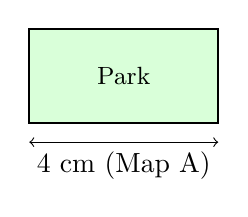
\begin{tikzpicture}[scale=0.6]
  \draw[thick,fill=green!15] (0,0) rectangle (4,2);
  \draw[<->] (0,-0.4) -- (4,-0.4);
  \node[below] at (2,-0.4) {$4$ cm (Map A)};
  \node at (2,1) {\small Park};
\end{tikzpicture}
\end{center}
\end{questionText}
\choiceA{$4$ cm}
\choiceB{$8$ cm}
\choiceC{$12$ cm}
\choiceD{$40$ cm}
\correctAnswer{C}
\explanation{Scale ratio: $\frac{30}{10} = 3$. New length: $4 \times 3 = 12$ cm on Map B.}
\end{practiceQuestion}

\begin{practiceQuestion}{6-2-q23}{gmc}
\begin{questionText}
The rectangle below is drawn at scale $1$ cm $= 8$ m. If the drawing is redrawn at $1$ cm $= 4$ m, what is the area of the new drawing?

\begin{center}
\begin{tikzpicture}[scale=0.6]
  \draw[thick,fill=funBlue!10] (0,0) rectangle (5,3);
  \draw[<->] (0,-0.4) -- (5,-0.4);
  \node[below] at (2.5,-0.4) {$5$ cm};
  \draw[<->] (5.4,0) -- (5.4,3);
  \node[right] at (5.4,1.5) {$3$ cm};
\end{tikzpicture}
\end{center}
\end{questionText}
\choiceA{$15$ cm$^2$}
\choiceB{$30$ cm$^2$}
\choiceC{$60$ cm$^2$}
\choiceD{$120$ cm$^2$}
\correctAnswer{C}
\explanation{Scale ratio: $\frac{8}{4} = 2$. New dimensions: $5 \times 2 = 10$ cm and $3 \times 2 = 6$ cm. New area: $10 \times 6 = 60$ cm$^2$.}
\end{practiceQuestion}

\begin{practiceQuestion}{6-2-q24}{gmc}
\begin{questionText}
A road on Map P is $9$ cm long (scale $1$ cm $= 6$ km). The same road appears as $3$ cm on Map Q. What scale does Map Q use?

\begin{center}
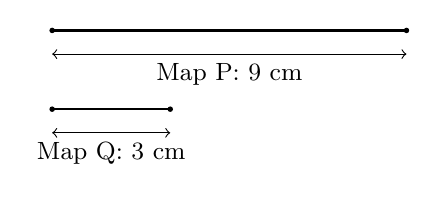
\begin{tikzpicture}[scale=0.5]
  % Map P
  \draw[thick] (0,2) -- (9,2);
  \fill (0,2) circle (2pt); \fill (9,2) circle (2pt);
  \draw[<->] (0,1.4) -- (9,1.4);
  \node[below] at (4.5,1.4) {\small Map P: $9$ cm};
  % Map Q
  \draw[thick] (0,0) -- (3,0);
  \fill (0,0) circle (2pt); \fill (3,0) circle (2pt);
  \draw[<->] (0,-0.6) -- (3,-0.6);
  \node[below] at (1.5,-0.6) {\small Map Q: $3$ cm};
\end{tikzpicture}
\end{center}
\end{questionText}
\choiceA{$1$ cm $= 2$ km}
\choiceB{$1$ cm $= 6$ km}
\choiceC{$1$ cm $= 12$ km}
\choiceD{$1$ cm $= 18$ km}
\correctAnswer{D}
\explanation{Actual road: $9 \times 6 = 54$ km. Map Q scale: $54 \div 3 = 18$ km per cm. Map Q uses $1$ cm $= 18$ km.}
\end{practiceQuestion}

% --- Graphical SA Questions (3) ---

\begin{practiceQuestion}{6-2-q25}{gsa}
\begin{questionText}
The triangle below is drawn at scale $1$ cm $= 5$ m. If the drawing is redrawn at $1$ cm $= 1$ m, find the new base length on the redrawn drawing.

\begin{center}
\begin{tikzpicture}[scale=0.7]
  \draw[thick,fill=funOrange!10] (0,0) -- (6,0) -- (3,3) -- cycle;
  \draw[<->] (0,-0.4) -- (6,-0.4);
  \node[below] at (3,-0.4) {$6$ cm};
\end{tikzpicture}
\end{center}
\end{questionText}
\correctAnswer{$30$ cm}
\explanation{Scale ratio: $\frac{5}{1} = 5$. New base: $6 \times 5 = 30$ cm.}
\end{practiceQuestion}

\begin{practiceQuestion}{6-2-q26}{gsa}
\begin{questionText}
A building is shown on Drawing X (scale $1$ cm $= 10$ m) as a rectangle $3$ cm wide and $5$ cm tall. If the building is redrawn at scale $1$ cm $= 5$ m, what is the perimeter of the new drawing?

\begin{center}
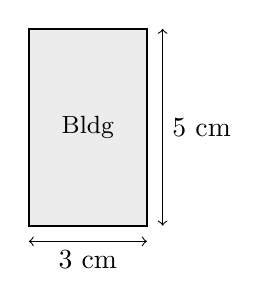
\begin{tikzpicture}[scale=0.5]
  \draw[thick,fill=gray!15] (0,0) rectangle (3,5);
  \draw[<->] (0,-0.4) -- (3,-0.4);
  \node[below] at (1.5,-0.4) {$3$ cm};
  \draw[<->] (3.4,0) -- (3.4,5);
  \node[right] at (3.4,2.5) {$5$ cm};
  \node at (1.5,2.5) {\small Bldg};
\end{tikzpicture}
\end{center}
\end{questionText}
\correctAnswer{$32$ cm}
\explanation{Scale ratio: $\frac{10}{5} = 2$. New dimensions: $3 \times 2 = 6$ cm and $5 \times 2 = 10$ cm. Perimeter: $2(6 + 10) = 32$ cm.}
\end{practiceQuestion}

\begin{practiceQuestion}{6-2-q27}{gsa}
\begin{questionText}
Map A shows a square lake as $4$ cm on each side at scale $1$ cm $= 50$ km. Map B shows the same lake at $2$ cm on each side. What scale does Map B use?

\begin{center}
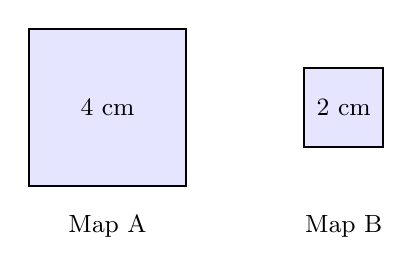
\begin{tikzpicture}[scale=0.5]
  \draw[thick,fill=blue!10] (0,0) rectangle (4,4);
  \node at (2,2) {\small $4$ cm};
  \node[below] at (2,-0.5) {\small Map A};
  \draw[thick,fill=blue!10] (7,1) rectangle (9,3);
  \node at (8,2) {\small $2$ cm};
  \node[below] at (8,-0.5) {\small Map B};
\end{tikzpicture}
\end{center}
\end{questionText}
\correctAnswer{$1$ cm $= 100$ km}
\explanation{Actual side: $4 \times 50 = 200$ km. Map B scale: $200 \div 2 = 100$ km per cm.}
\end{practiceQuestion}
